\documentclass[12pt]{article}

\usepackage[margin=1in]{geometry}
	%changes default margins

\usepackage{setspace}
\singlespacing
	%\singlespacing,\onehalfspacing,\doublespacing can be set and everything thereafter will use that spacing. You can switch within the document as often as you wish
	
\usepackage{parskip}
%changes paragraphs to have an extra space and new indentation with paragraphs, rather than indenting every new paragraph. This is completely a stylistic choice and neither is better than the other.


\usepackage{mathtools,amssymb} %useful math stuff. there are a lot of ams* packages. If you have a math need, it's probably in there

	
	
%\usepackage{natbib}
%\usepackage{biblatex} %natbib is older and available from almost all journals, biblatex is not, but biblatex has more flexibility and options.

%\usepackage[natbib=true]{biblatex} %this often works and requires minimal changes 

%for biblatex you write \textcite{citekey} and \parencite{citekey}
%for natbib you write \citet{citekey} and \citep{citekey}. Please avoid using \cite{} since you won't control whether it's parenthetical, but you are responsible for whether you use something in text or parenthetically.
%for \usepackage[natbib=true]{biblatex} you follow the natbib style and you won't have to perform search/replaces in your document, you would only need to change the package call and bibliography call.

\usepackage{natbib}
\bibliographystyle{chicago}

%other useful packages
% \usepackage{graphicx} %for including images including pdf
\usepackage{booktabs} % for tables
\usepackage{siunitx} % for longitude and latitude degrees


\title{Using Machine-Learning Methods to Improve Air Temperature prediction from the Outputs of a Numerical Weather Prediction
Model}
\date{\today}

\begin{document}
	
\maketitle
	
\section*{Abstract}
\section{Introduction}
\section{Literature review}

An atmospheric reanalysis involves retrospectively describing the atmospheric state by assimilating observations into an atmospheric model simulation using data assimilation techniques. Reanalysis products provide a consistent and continuous description of the atmospheric state over a relatively long period, typically spanning 40 to 70 years, and are particularly valuable in regions where observational data are sparse (\cite{Jung2016}). These products are widely used to estimate past and present atmospheric conditions over the world (\cite{Large2009,Tsujino2018}).

However, due to the limitation of the implemented numerical models, errors may occur, especially in regions with shallow atmospheric boundary layers and temperature inversions, which are challenging features for models to simulate accurately (\cite{Zampieri2018}). Previous studies have identified significant surface temperature biases in most reanalysis products over the world, primarily attributed to inaccuracies in representing the snow and sea ice state. Future reanalysis versions are expected to address these deficiencies by incorporating fully coupled modeling systems and assimilating new types of near-surface observations. 

This study explores the use of machine learning algorithms to correct the surface temperature data of GDAS/FNL. GDAS/FNL stands for Global Data Assimilation System/Final Analysis, which is operated by the National Centers for Environmental Prediction (NCEP) in the United States to generate global atmospheric analysis data. GDAS/FNL data are produced by assimilating data from various observational sources (such as satellite observations, surface stations, aircraft probes, etc.) using data assimilation techniques to provide high-quality meteorological field data for various regions worldwide. 

Many scholars have conducted corrections on reanalysis data by machine learning algorithms. \cite{Zampieri2023} used machine learning to correct various datasets and the correction leads on average to a 27\% temperature bias reduction for ERA5 and 7\% for JRA-55 if compared to independent in situ observations from the MOSAiC campaign (respectively, 32\% and 10\% under clear-sky conditions). \cite{Hou2022} applied LDA correction to ERA5 data, and compared with ERA5 and station observation data, the results show that the root mean square error can be reduced by 2\%–4\% and the correlation coefficient can be increased by 1\%–5\% for different lead times, with the most distinct improvement effect for the medium-term forecast time.

In our study, the correction model is trained using surface observations. This approach aims to improve the realism of surface temperature estimates over Toronto regions. 

\section{Data and methodology}

In this project, we explored three different dataset, the first two are combined used as our correction methodologies for a global weather model using local data, the third dataset is a local dataset to test the time series forcasting model on a local scale.

\subsection{Data}

The following sections present some brief introductories of each data set we used, the key variables included in each data set, and how we do the data preprocessing.

\subsubsection{NCEP}

The NCEP (National Centers for Environmental Prediction) Global Forecast System (GFS) model is a numerical weather prediction system operated by the National Weather Service (NWS) of the United States. It is one of the major global models used for weather forecasting worldwide. The GFS model utilizes complex mathematical equations to simulate the behavior of the atmosphere and predict future weather conditions.

The GFS model generates forecasts for a wide range of atmospheric variables including temperature, humidity, wind speed and direction, precipitation, and pressure at various levels of the atmosphere (As shown in Table~\ref{tab:GFS}). These forecasts are produced for different time ranges ranging from short-term forecasts (hours to a few days) to medium-range forecasts (up to two weeks or more).

\begin{table}[htbp]
    \centering
    \caption{NCEP GFS Model Key Features}
    \begin{tabular}{@{}ll@{}}
        \toprule
        \textbf{Parameter} & \textbf{Description} \\
        \midrule
        Air Temperature & Temperature of the air in degrees Celsius or Fahrenheit \\
        Wind Speed & Speed of the wind in meters per second or miles per hour \\
        Precipitation & Amount of precipitation in millimeters or inches \\
        Relative Humidity & Percentage of moisture in the air relative to saturation \\
        Pressure & Atmospheric pressure in hectopascals or millibars \\
        Cloud Cover & Fraction of the sky covered by clouds \\
        \bottomrule
    \end{tabular}
    \label{tab:GFS}
\end{table}

The model ingests observational data from various sources including weather stations, satellites, radar, and aircraft to initialize the simulation of the atmosphere. It then uses sophisticated numerical techniques to solve the equations of fluid motion, thermodynamics, and other physical processes that govern atmospheric behavior.

The output from the GFS model is used by meteorologists and weather forecasters to generate weather forecasts, issue warnings for severe weather events, and provide guidance for various sectors including agriculture, transportation, energy, and emergency management.

In our model, our predictions is the corrections of air temperature output of GFS model. GFS model simulate atmospheric processes on a grid system. The precision of the grid is determined by the spacing of grid points in both horizontal and vertical dimensions. Higher precision grids have smaller spacing between grid points, allowing for more detailed representation of atmospheric features and processes. In our case, we selected a specific grid with 1 degree Based on that value and the locally collected data, we train a calibration model to improve the local air temperature prediction.

\subsubsection{DACCD}

For local temperature data, we use data from the Digital Archive of Canadian Climatological Data (DACCD). It is a comprehensive repository of historical climatological information specific to Canada. Managed by Environment and Climate Change Canada (ECCC), the DACCD houses a vast collection of meteorological data spanning several decades, including observations of temperature, precipitation, wind patterns, atmospheric pressure, and other relevant climatic variables (As shown in Table~\ref{tab:DACCD}). This data is sourced from various observation stations, weather monitoring networks, and research initiatives conducted throughout Canada's vast geographic landscape.

\begin{table}[htpb]
	\centering
	\caption{Key features in the DACCD dataset}
	\label{tab:DACCD}
	\begin{tabular}{lll}
		\hline
	 Variables & Symbol & Unit\\
		\hline
	Longitude & x & deg\\
	Latitude & y & deg\\
	Daily mean temperature & Mean Temp & degC\\
	Daily max temperature & Max Temp & degC\\
	Daily min temperature & Min Temp & degC\\
	Daily total rainfall & Total Rain & mm\\
	Daily total snowfall & Total Snow & cm\\
	Daily total precip & Total Precip & mm\\
	Snow on the Ground& Snow on Grnd & cm\\
	Direction of extreme gust & Dir of Max Gust & 10's of deg\\
	Speed of extreme gust & Spd of Max Gust & km/h\\
	\hline
	\end{tabular}
\end{table}

The climatological data in the DACCD dataset are stored at five distinct intervals: minutely, every fifteen minutes, hourly, daily, or monthly. For this project, we specifically utilize the daily data for analysis and modeling purposes.


Weather station selection: The blue box in Figure~\ref{Fig:stations} shows one grid in the GFS model. It bounds a latitude from \ang{43.00} N to \ang{44.00}N, and a longitude from \ang{-79.00} E to \ang{-80.00} E. Using this boundary, we can select all weather stations whose location falls into this grid. In total we got 291 weather stations. However, not all stations are currently in operation. Therefore, we filtered out all operating weather stations from year 2016 to 2023 in this grid, which end up with only 11 stations marked in red location pins in Figure~\ref{Fig:stations}.

Among the 11 selected weather stations, not all of which are 

\begin{figure}[htpb]
	\centering
	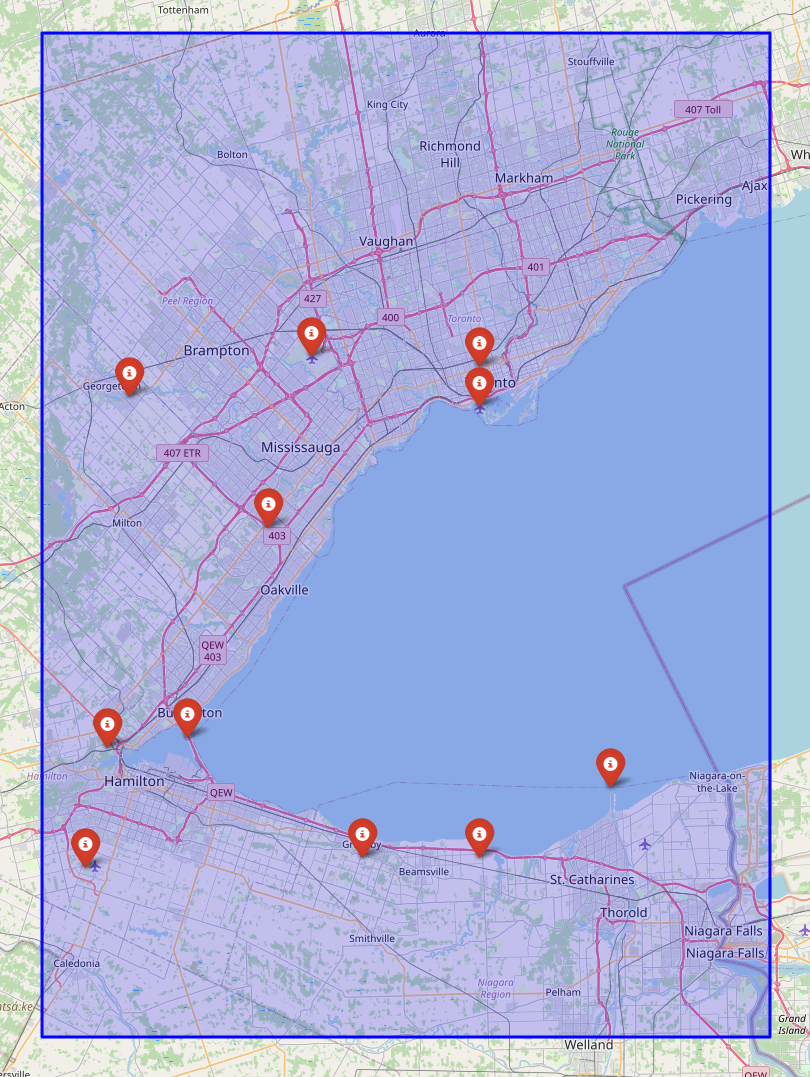
\includegraphics[width=0.8\textwidth]{pic/stations.png}
	\caption{Weather stations used in this project}
	\label{Fig:stations}
\end{figure}

\subsubsection{Jena Weather dataset}

The Max-Planck-Institute for Biogeochemistry, located in Jena, Germany, provides a comprehensive weather dataset encompassing various meteorological parameters. This dataset spans a significant period, with measurements collected every 10 minutes, starting from the year 2003. It comprises 14 distinct features, including crucial metrics such as air temperature, atmospheric pressure, and humidity. Details shown in Table~\ref{tab:Jena}.

To ensure computational efficiency and focus on a specific timeframe, we will narrow down our analysis to the data collected between the years 2009 and 2016. This time span offers a substantial duration for observation while maintaining computational manageability.

\begin{table}[htpb]
	\centering
	\caption{Key features within the Jena dataset}
	\label{tab:Jena}
	\begin{tabular}{lll}
		\hline
		Variables & Symbol & Unit\\
		\hline
	Atmospheric pressure & p & mbar\\
	Air temperature & T & degC\\
	Potential temperature & Tpot & K\\
	Dew point temperature & Tdew & degC\\
	Relative humidity & rh & \%\\
	Saturation water vapor pressure & VPmax & mbar\\
	Actual water vapor pressure & VPact & mbar\\
	Water vapor pressure deficit & VPdef & mbar\\
	Specific humidity & sh & g/kg\\
	Water vapor concentration & H2OC & mmol/mol\\
	Air density & rho & g/m**3 \\
	Wind velocity & wv & m/s\\
	Maximum wind velocity & max. wv & m/s\\
	Wind direction & wd & deg\\
		\hline
	\end{tabular}
\end{table}


This comprehensive set of features facilitates in-depth analysis and modeling of various atmospheric and environmental phenomena, providing valuable insights into climate patterns, ecosystem dynamics, and biogeochemical processes over the specified time period.
\subsection{Methodology}

The aim here is to model the average air temperature at the above-mentioned meteorological stations in Toronto from the outputs of the NCEP GFS Model, building on the work of \cite{Goutham2021}.

Here, the target variable is the observed air temperature and explanatory variables derive only from the history records from Toronto. (p=8 explanatory variables: Mean Temp (°C),Max Temp (°C),Min Temp (°C),Total Rain (mm),Total Snow (cm),Total Precip (mm) and Snow on Grnd (cm).

In the realms of statistics and machine learning, two primary methodologies are commonly employed: parametric and non-parametric approaches. Parametric models entail defining the relationship between outputs and inputs analytically, often based on specific probability distributions such as the Gaussian model. In contrast, non-parametric methods do not hinge on assuming a particular data distribution but instead entail the adjustment of multiple tuning parameters.

\subsubsection{Linear Regression}

Linear regression is a commonly used model, which gives a linear relationship between explanatory and the response variable. In our work, the response variable is $Y_t$ and the explanatory variables goes from $X_{t-d}^1, X_{t-d}^2,\ldots,X_{t-d}^p$ at a given time $t$ and previous $d$ days history.

\begin{equation}
	Y_{t} = \beta_0+\sum_{j=1}^p \beta_j X_{t-d}^j + \epsilon_t
\end{equation}

where the coefficient $\beta_j$ are the regression coefficients estimated using a least-squares approach, and $\epsilon$ is the error. We use $d=1$ in our model.

For a large number of variables, in order to obtain a precise estimation, it is necessary to select the most relevant variables. Many methods are available, either forwards or backwards, to retain only a subset of the explanatory variables. Forwards selection starts with an empty list of predictors adding one highly significant predictor at each step until a stopping criterion is reached, whereas backwards selection starts with a full list of predictors eliminating one highly insignificant predictor at each step until a stopping criterion is reached. Omitting the Gaussian assumption, Lasso regression (also called $\mathcal{L}^1$ regularization) may be employed to select the most important predictors by adding a penalty term to the least-squares error (\cite{ISL2}; \cite{Tibshirani1996}). This penalty acts as a constraint favouring a weaker sum of the absolute values of the regression coefficients; this results in some of the coefficients reducing to zero, implying that the corresponding explanatory variable is dropped.


\section{Results and discussion}

\subsection{Linear Regression Model}
\subsubsection{Variable selection}
\subsubsection{Cross Validation}

\begin{figure}[htpb]
	\centering
	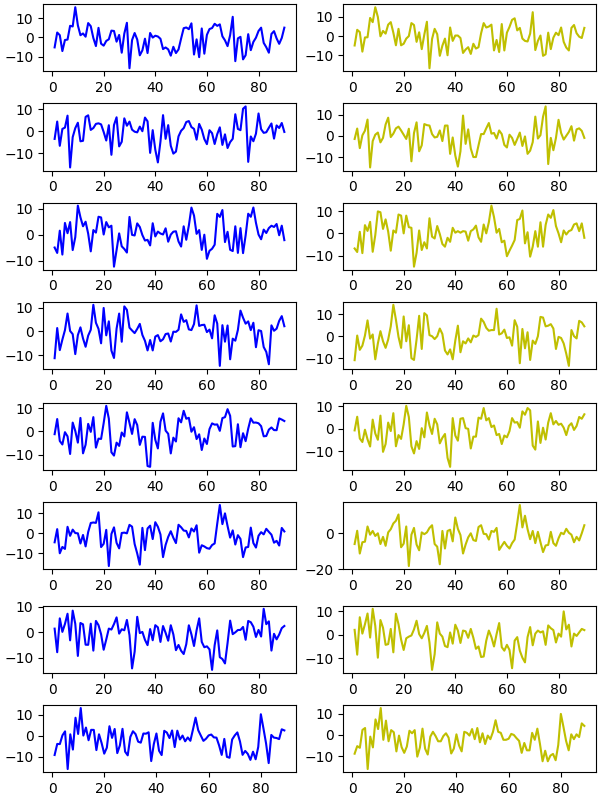
\includegraphics[width=0.8\textwidth]{pic/Predicted-and-Tested_1.png}
	\caption{Prediction: January to March}
	\label{Fig:pred-1}
\end{figure}

\begin{figure}[htpb]
	\centering
	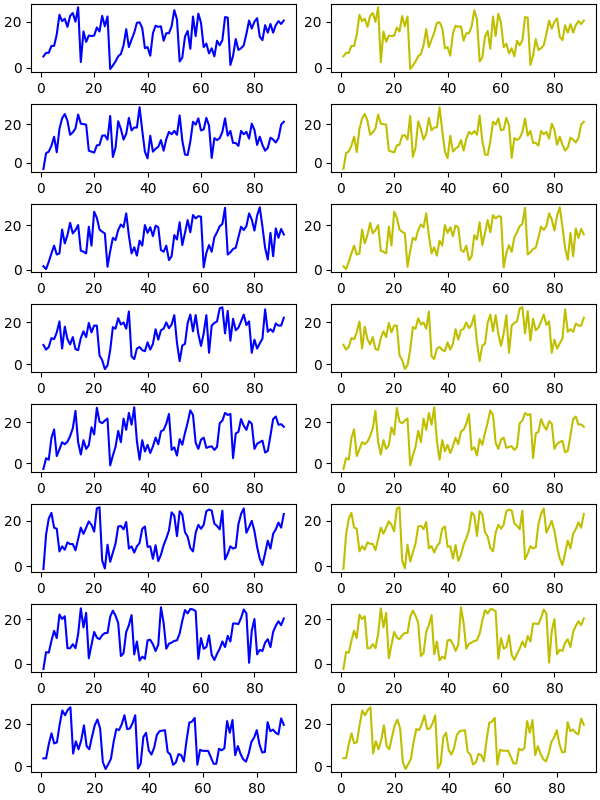
\includegraphics[width=0.8\textwidth]{pic/Predicted-and-Tested_2.png}
	\caption{Prediction: April to June}
	\label{Fig:pred-2}
\end{figure}

\begin{figure}[htpb]
	\centering
	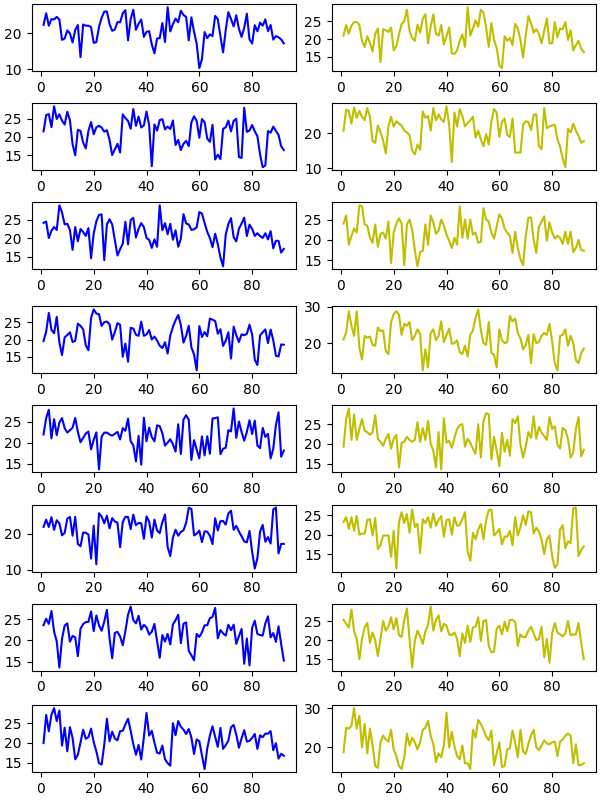
\includegraphics[width=0.8\textwidth]{pic/Predicted-and-Tested_3.png}
	\caption{Prediction: July to September}
	\label{Fig:pred-3}
\end{figure}

\begin{figure}[htpb]
	\centering
	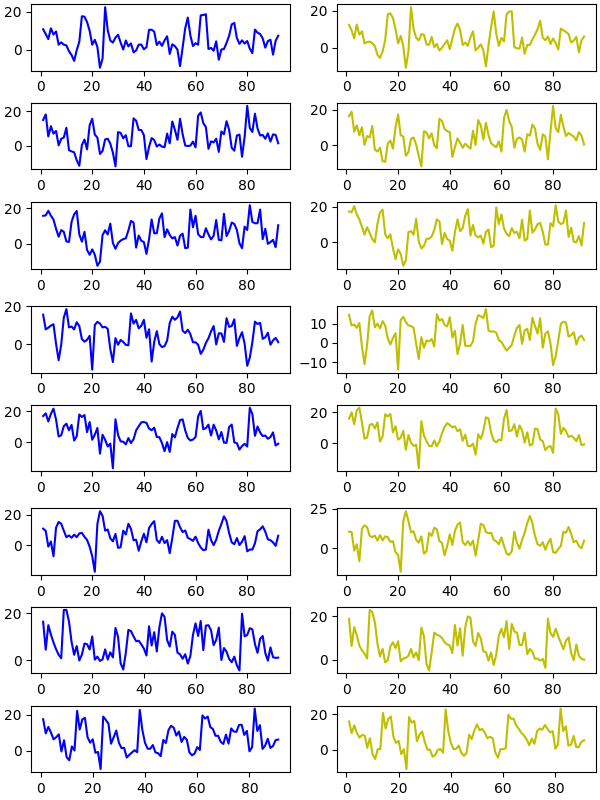
\includegraphics[width=0.8\textwidth]{pic/Predicted-and-Tested_4.png}
	\caption{Prediction: October to December}
	\label{Fig:pred-4}
\end{figure}

\section{Conclusion}

\bibliography{cite}

\end{document}

